%Dave's handout 1.7 intro 2nd derivatives
%Dave's handout 2.2 2nd derivative rule
\vspace{-0.25 in}
\begin{framed}
\subsection*{Objectives}
\begin{itemize}
    \item Explain how the sign of the first derivative affects the shape of a function’s graph.
    \item Using the first derivative of a function $f$, determine interval(s) where $f$ is increasing and is decreasing.
    \item Using the graph of a function $f$, determine critical value(s) of $f$.
    \item Using the formula of a function $f$, determine critical value(s) of $f$.
    \item Using the first derivative of a function $f$ and its critical value(s), determine local extreme values(s).
\end{itemize}

%%%Reading Assignment%%%
\subsection*{Suggested Reading:}
\begin{itemize}
\item \cite{Calaway}\footnotemark[1]
   \begin{itemize}
        \item \emph{Section 2.7 Optimization}
    \end{itemize}
\item \cite{openstax}\footnotemark[2]
    \begin{itemize}
        \item \emph{Section 4.3  Maxima and Minima}
        \item \emph{Section 4.5 Derivatives and teh Shape of a Graph}
    \end{itemize}
\item \cite{activeCalc}\footnotemark[3]
    \begin{itemize}
        \item \emph{Section 3.1 Using derivatives to identify extreme values}
    \end{itemize}
\end{itemize}
%\subsection*{Supplemental Materials:}
%%%Key Terms%%%
\subsection*{Key Terms and Concepts:} 

\begin{multicols}{2}
\begin{itemize}
    \item Critical Numbers
    \item Sign Chart
    \item First Derivative Test
    \item Local Extreme Value(s) (Local Extremum (Extrema)
    \item Local Maximum and Local Minimum
\end{itemize}
\end{multicols}
\end{framed}
\footnotetext[1]{Available free to download from \url{http://www.opentextbookstore.com/details.php?id=14} .}
\footnotetext[2]{Available free to download from \url{https://openstax.org/details/books/calculus-volume-1}.}
\footnotetext[3]{Available free to download from \url{https://activecalculus.org/single/frontmatter.html}.}

\newpage
%%%%%%%%%%START LESSON CONTENT%%%%%%%%%%%%%
%\noindent\makebox[\linewidth]{\rule{\textwidth}{0.8pt}}
\Opensolutionfile{ans}[ans8]
\Opensolutionfile{ansL}[ansL8]
%%%%%%%%%%%%%%%%Start First Topic%%%%%%%%%%%%%%%%%%%%%%%%%%%%%
\noindent Without calculus, we only know how to find the optimum points in a few specific examples (for example, we know how to find the vertex of a parabola). But what if we need to optimize an unfamiliar function?\\
The best way we have without calculus is to examine the graph of the function, perhaps using technology. But our view depends on the viewing window we choose – we might miss something important. In addition, we’ll probably only get an approximation this way. (In some cases, that will be good enough.)\\
Calculus provides ways of drastically narrowing the number of points we need to examine to find the exact locations of maximums and minimums, while at the same time ensuring that we haven’t missed anything important.\\
Before we examine how calculus can help us find maximums and minimums, we need to be familiar with the vocabulary and the concepts we will develop and use to describe \textbf{behavior of a function}.\\

\begin{tcolorbox}[title = {Increasing and Decreasing Functions in an interval}]
    Simply put, if there is some interval of values of x for which the value of a function is getting larger as we move from left to right, we say that the function is increasing in that interval.  A decreasing function is defined similarly, with the value of the function becoming smaller vs. larger.\\\\
    For a function \(f\) which is \emph{differentiable}\footnotemark on an interval \(I\):
\renewcommand{\labelenumii}{\roman{enumii}}
\begin{enumerate}
    \item if \(f'(x)>0\) for all \(x\) in the interval \(I\), then \(f\) is \textbf{increasing} on \(I\).
     \item if \(f'(x)<0\) for all \(x\) in the interval \(I\), then \(f\) is \textbf{decreasing} on \(I\).
      \item if \(f'(x)=0\) for all \(x\) in the interval \(I\), then \(f\) is \textbf{constant} on \(I\).
\end{enumerate}
\end{tcolorbox}

\noindent The derivative of a function tells about the general shape of the function, and we can use that shape information to determine if an extreme point is a maximum or minimum or neither (See Figure \ref{fig:dervBeh2}).

\begin{figure}[h]
    \centering
    \caption{} \footnotemark
    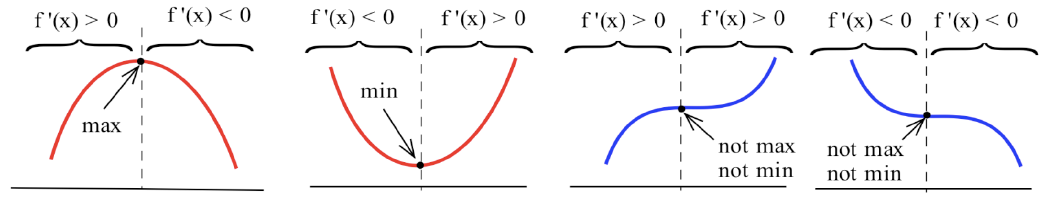
\includegraphics[width=0.95\textwidth]{derivatives-functions/derivativeBehavior} 
    \label{fig:dervBeh2}
\end{figure}

\footnotetext[1]{See Lesson \ref{differentiability}: Differentiability and Continuity}
\footnotetext[2]{From \cite{Hoffman} ;  page 88}

\subsection*{Local Extreme Points}

\begin{tcolorbox}[title = {Local Extreme Points }]
\begin{itemize}[leftmargin=*]
    \item A \textbf{local maximum} point is a point on the graph of the function at which the function changes from an increasing function to a decreasing function. A point is a local maximum if it is \underline{higher than} all the \textbf{nearby points}. Formally, we say
    \begin{itemize}
        \item $f$ has a \textbf{local maximum} at $c$ if $f(c)\ge f(x)$ for all $x$ near $c$.
    \end{itemize}
    \item A \textbf{local minimum} point is a point on the graph of the function at which the function changes from a decreasing function to an increasing function. A point is a local minimum if it is \underline{lower than} all the \textbf{nearby points}. Formally, we say
    \begin{itemize}
        \item $f$ has a \textbf{local minimum} at $c$ if $f(c)\le f(x)$ for all $x$ near $c$.
    \end{itemize}
\end{itemize}
\end{tcolorbox}
\vspace{-0.5cm}
\subsubsection*{Notes:}
\begin{itemize}
    \item These points are also referred to as “relative” maximum and minimum points.
    \item $f$ has a \textbf{local extremum} at $c$ if $f(c)$ is a local maximum or minimum. The plural of local extremum is \textbf{local extrema}.
    \item The plurals of these are \textbf{maxima} and \textbf{minima}. We often simply say \textbf{“max”} or \textbf{“min”}.
\end{itemize}

\subsection*{Critical Number}
\begin{tcolorbox}[title = {Critical Number }]
\begin{itemize}[leftmargin=*]
    \item A \textbf{critical number} of a function $f$ is a number $c$ for which either $f'(c)=0$ or $f'(c)$ is undefined \underline{AND $c$ is in the domain of $f$}.
    \item A \textbf{critical point} of a function $f$ is a point $(c,f(c))$ where $c$ is a critical number of $f$.
\end{itemize}
\end{tcolorbox}
\vspace{-0.5cm}
\subsubsection*{Notes:}
\begin{itemize}
    \item A local max or min of $f$ can only occur at a critical point.
    \item The critical numbers only give the \textbf{possible} locations of extremes, and some critical numbers are not the locations of extremes.
    \begin{figure}[h]
    \centering
    \caption{From left to right, a function with a relative maximum where its derivative is zero; a function with a relative maximum where its derivative is undefined; a function with neither a maximum nor a minimum at a point where its derivative is zero; a function with a relative minimum where its derivative is zero; and a function with a relative minimum where its derivative is undefined.} 
    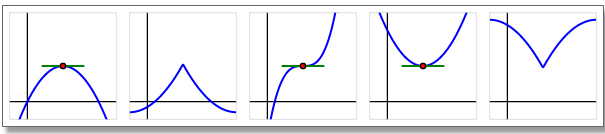
\includegraphics[scale=2]{images/FirstDerivativeTest/ActiveCalculus3_1_criticalNumbers.PNG} 
    \label{fig:oneLocalExtrema}
\end{figure}
    
\end{itemize}
\newpage
%%%%%%%%%%%%%%%%%%%%%%%%%%%%%%%%%%%%%%

%%% Question 11 from https://www.math.tamu.edu/~mayaj/m142_Chapter5_Sec5.1.pdf%%%
\begin{example}
Use the graph of the function $f(x)$ displayed below to answer the following questions.
\begin{figure}[h]
    \centering
    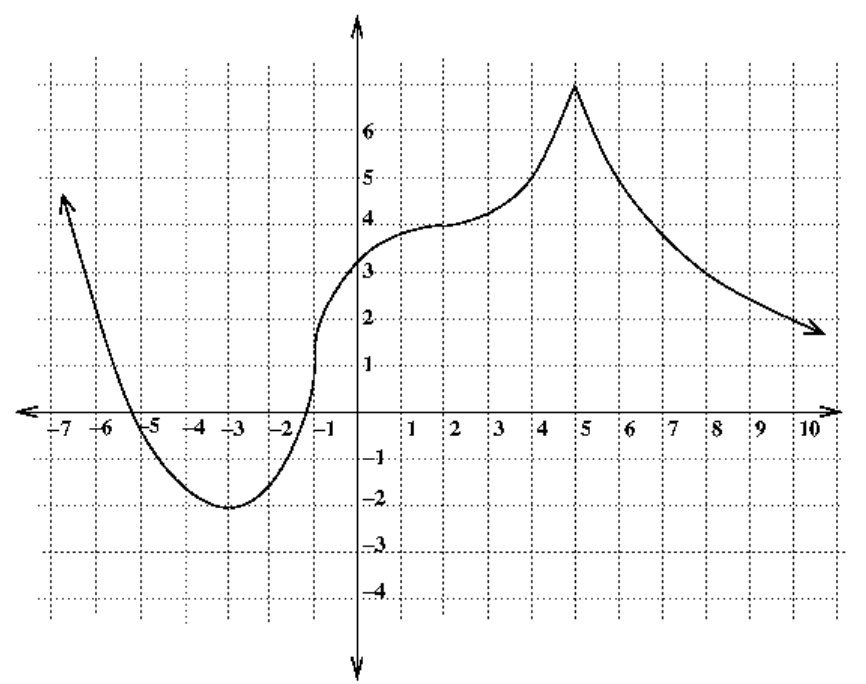
\includegraphics[width=0.6\textwidth]{images/optimization/exampleGraph1.png}
    \label{fig:my_label}
\end{figure}
\renewcommand{\labelenumi}{(\alph{enumi})}
\begin{enumerate}[leftmargin=*]
    \item Determine all intervals on which $f(x)$ is \textbf{increasing}.\vspace*{\stretch{1}}
    \item Determine all intervals on which $f(x)$ is \textbf{decreasing}.\vspace*{\stretch{1}}
    \item Find the critical values where $f'(x)$ does not exist.\vspace*{\stretch{1}}
    \item Find the critical values where $f'(x)=0$.\vspace*{\stretch{1}}
    \item Find the $x-$coordinate(s) of the relative maxima for $f(x)$. \vspace*{\stretch{2.5}}
    \item Find the $x-$coordinate(s) of the relative minima for $f(x)$. \vspace*{\stretch{1}}
\end{enumerate}
    %%short answer
    \begin{sol}
    (a) $x=-1,5$ (b) $x=-3,2$ (c) $x=5$ (d) $x=-3$
    \end{sol}
    %%solution
    \begin{solL}
    Complete solution here.....
    
    \end{solL}
    
\end{example}

\newpage
%%%%%%%%%%%%%%%%%%%%%%%%%%%%%%%%%%%%%%%%%
\begin{tcolorbox}[title = {The First Derivative Test for Extremes:}]

Suppose that $c$ is a \textbf{critical number} of a continuous function $f$. For each critical number $c$, examine the sign of $f'$ to the left and to the right of $c$. What happens to the sign as you move from left to right?
\renewcommand{\labelenumi}{(\alph{enumi})}
\begin{enumerate}[leftmargin=*]

    \item If $f'(x)$ changes from \textbf{positive to negative} at $c$, then $f$ has a \textbf{local max} at $(c,f(c))$.
    \item If $f'(x)$ changes from \textbf{negative to positive} at $c$, then $f$ has a \textbf{local min} at $(c,f(c))$.
    \item If $f'(x)$ \textbf{does not change sign} at $c$, then $(c,f(c))$ is \textbf{neither} a local max nor a local min.
\end{enumerate}
\end{tcolorbox}

\begin{tcolorbox}[title={Steps for finding where $f$ is Increasing/Decreasing or any Local Extrema}]
\begin{enumerate}[leftmargin=*]
    \item Find the \textbf{domain} of $f$.
    \item Find all \textbf{critical numbers} of $f$.
    \item Make a \textbf{sign chart} to track where $f'>0$ or $f'<0$ by following these steps:
    \renewcommand{\labelenumii}{(\roman{enumii})}
    \begin{enumerate}
        \item Plot all critical number(s) on a number line, and all other $x-$values that are not in the domain but are providing $f'(x)=0$ or $f'(x)$ undefined.
        \item Choose $x-$values to test regions on the number line around the numbers plotted on the number line.
        \item Plug test values into $f'$ and record the sign $(\pm)$
    \end{enumerate}
    \item Determine any \textbf{local extrema} using the \emph{First Derivative Test for Extremes}.
\end{enumerate}
\end{tcolorbox}


%% Question 9 from https://www.math.tamu.edu/~mayaj/m142_Chapter5_Sec5.1.pdf%%%
\begin{example}
Given the function $f(x)=\displaystyle\frac{x^2+3}{x-1}$ and its first derivative is shown below:
\begin{equation*}
    f'(x)=\frac{(x-3)(x+1)}{(x-1)^2}
\end{equation*}
Answer the following questions.
\renewcommand{\labelenumi}{(\alph{enumi})}
\begin{enumerate}[leftmargin=*]
    \item Find the domain of $f$.\vspace*{\stretch{1.5}}
    \item Find the critical number(s) of $f$. \vspace*{\stretch{1}}
    \newpage
    \item Make a sign chart for the function and use the chart to find the following:
    \renewcommand{\labelenumii}{(\roman{enumii})}
    \begin{enumerate}
        \item all intervals on which $f(x)$ is increasing.
        \item all intervals on which $f(x)$ is decreasing.
        \item the $x-$coordinate(s) of all relative extrema on the graph of $f(x)$. 
    \end{enumerate}
    \vspace*{\stretch{1}}
\end{enumerate}
    %%short answer
    \begin{sol}
    (a) $(-\infty,1)\cup (1,\infty)$ (b) $x=-1;x=1;x=3$ (c) $x=-1;x=3$ (d)(i) $(-\infty,-1)\cup (3,\infty)$ (d)(ii) $(-1,1)\cup (1,3)$ (d)(iii) local max at $x=-1$; local min at $x=3$
    \end{sol}
    %%solution
    \begin{solL}
    Complete solution here.....
    
    \end{solL}
    
\end{example}

%%%Example: Dave's handout 2.3 Derivatives: Behavior and graph of a function%%%
\begin{example}
For each of the following functions, determine all \textbf{local extrema} using the \emph{First Derivative Test}. \textbf{Include a sign chart}.
\renewcommand{\labelenumi}{(\alph{enumi})}
\begin{enumerate}[leftmargin=*]
    \item $f(x)=\displaystyle\frac{1}{3}x^3-\frac{5}{2}x^2+4x$. %%OpenStax; 4.3 Maxima and Minima; ex.4.12a
    \begin{figure}[h!]
        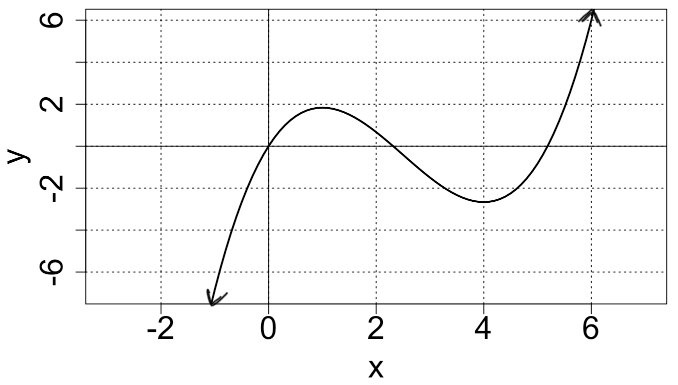
\includegraphics[width=0.45\textwidth,inner]{images/optimization/exampleGraph2.png}
        \label{fig:exampleGraph2}
    \end{figure}
    \vspace*{\stretch{1}}
    \newpage
    \item $f(x)=(x^2-1)^3$. %%OpenStax; 4.3 Maxima and Minima; ex.4.12b
    \begin{figure}[h!]
        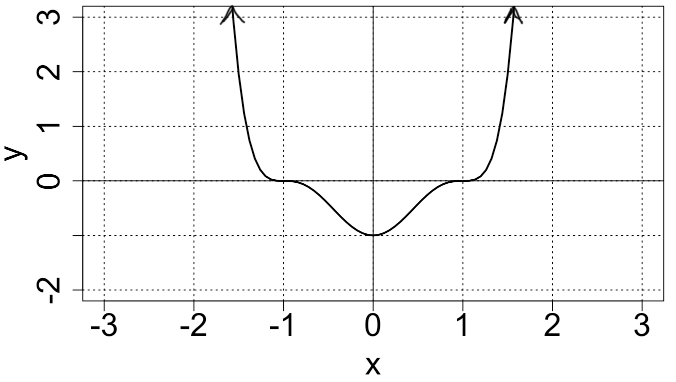
\includegraphics[width=0.45\textwidth,inner]{images/optimization/exampleGraph3.png}
        \label{fig:exampleGraph3}
    \end{figure}
    \vspace*{\stretch{1}}
    \item $f(x)=x+\displaystyle\frac{100}{x-1}$.\label{1stDervTestLocal_ex7}  %%%Example: Dave's handout 2.3 Derivatives: Behavior and graph of a function%%%
    \begin{figure}[h!]
        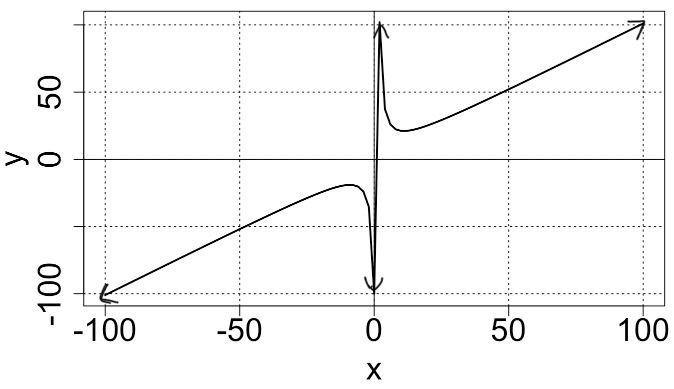
\includegraphics[width=0.45\textwidth,inner]{images/optimization/exampleGraph4.png}
        \label{fig:exampleGraph4}
    \end{figure}
     \vspace*{\stretch{1}}
    \item $f(x)=\displaystyle\frac{10}{x+2}$. %%%Example: Dave's handout 2.3 Derivatives:Behavior and graph of a function%%%
    \begin{figure}[h!]
        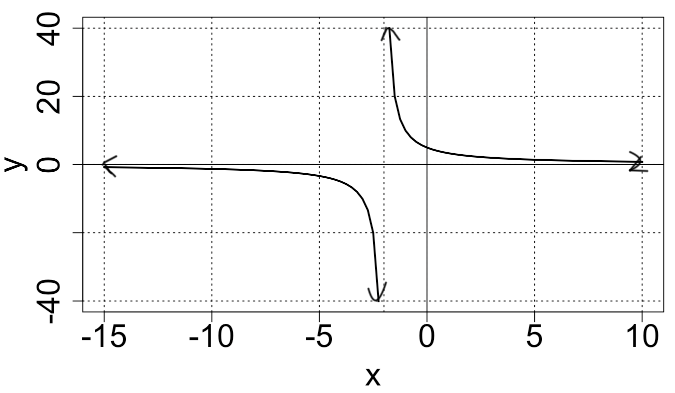
\includegraphics[width=0.45\textwidth,inner]{images/optimization/exampleGraph5.png}
        \label{fig:exampleGraph5}
    \end{figure}
     \vspace*{\stretch{1}}
\end{enumerate}
    %%short answer
    \begin{sol}
    (a) local max at $x=1$;local min at $x=4$. (b) local minimum at $x=0$. (c) local max at $x=-9$; local min at $x=11$. (d) no local extrema.
    \end{sol}
    %%solution
    \begin{solL}
    Complete solution here.....
    
    \end{solL}
    
\end{example}




%%%%%%%%%%%%%%%End Lesson%%%%%%%%%%%%%%%%%%
\Closesolutionfile{ans}
\Closesolutionfile{ansL}

%%%Short Answers to Examples%%%
%\vspace*{\fill}
\subsection*{Short Answers to Examples}
%\vspace{-0.25cm}

\input{ans8}



